\documentclass[12pt,a4paper]{article}

\usepackage[utf8]{inputenc}
\usepackage[T1]{fontenc}
\usepackage[brazil]{babel}
\usepackage{amsmath,amssymb}
\usepackage{geometry}
\usepackage{booktabs}
\usepackage{graphicx}
\usepackage[hypertexnames=false]{hyperref}
\usepackage{float}

\geometry{margin=2.5cm}

\title{
Fichamento Teórico e Experimental\\
\large Wavelet Packet Transform (WPT)\\
PIBITI -- Mês 2
}

\author{Thiago Mateus Schiavi\\
Fatec Ourinhos}

\date{Outubro de 2026}

\begin{document}

\maketitle
\tableofcontents
\newpage

\section{Introdução}

Este documento apresenta os fundamentos da transformada
Wavelet Packet Transform (WPT) e os experimentos iniciais
realizados no projeto PIBITI de detecção de deepfakes
de áudio em português brasileiro.

Os experimentos utilizam áudios do corpus BRSpeech-DF,
padronizados para WAV, 16 kHz e mono.


\section{Corpus e protocolo experimental}

O projeto utiliza o corpus BRSpeech-DF, composto por gravações
reais (\textit{bona fide}) e sintéticas (\textit{spoof}) em
português brasileiro.

Foi preparado um subconjunto piloto de 600 áudios,
distribuídos igualmente entre as classes e as partições
oficiais de treino, validação e teste.

Os sinais foram padronizados para WAV, mono, 16 kHz e PCM
de 16 bits.

Para investigar a separação dos locutores, foram analisados
76.644 registros reais presentes em 40 arquivos Parquet.
Foram encontrados 62 identificadores distintos: 42 no treino,
10 na validação e 10 no teste.

Não houve sobreposição desses identificadores entre as
partições. Os identificadores foram extraídos do prefixo
dos nomes dos arquivos, seguindo a hipótese de que esse
prefixo representa o locutor.

A identidade dos locutores nos registros sintéticos não foi
verificada diretamente. Portanto, a análise não comprova
isoladamente a ausência de vazamento de locutores em todo
o corpus.

\section{Fundamentação da WPT}

A Wavelet Packet Transform permite decompor um sinal
em múltiplas sub-bandas, oferecendo uma representação
tempo-frequência.

Diferentemente da transformada wavelet discreta
tradicional, a WPT decompõe tanto os coeficientes
de aproximação quanto os de detalhe.

No nível $L$, uma árvore completa possui:

\begin{equation}
N = 2^L
\end{equation}

Portanto:

\begin{itemize}
\item $L=4$: 16 sub-bandas.
\item $L=5$: 32 sub-bandas.
\end{itemize}

\section{Wavelets-mãe}

Foram consideradas três wavelets-mãe:

\begin{itemize}
\item Daubechies 4 (db4).
\item Daubechies 8 (db8).
\item Symlet 8 (sym8).
\end{itemize}

A db4 apresenta filtro de decomposição com
8 coeficientes, enquanto db8 e sym8 possuem
16 coeficientes.

\section{Decomposição e reconstrução}

A decomposição foi realizada inicialmente com
a wavelet db4 e nível $L=4$.

Foram obtidas 16 sub-bandas e realizada a
reconstrução completa do sinal.

A qualidade da reconstrução foi avaliada pelo
erro quadrático médio:

\begin{equation}
MSE = \frac{1}{N}
\sum_{n=1}^{N}
(x[n]-\hat{x}[n])^2
\end{equation}

O experimento apresentou:

\begin{itemize}
\item Amostras originais: 127.275.
\item Amostras reconstruídas: 127.275.
\item MSE: $2{,}6771 \times 10^{-34}$.
\item Erro máximo: $2{,}2204 \times 10^{-16}$.
\end{itemize}

A soma das 16 sub-bandas reconstruídas individualmente
também recuperou o sinal com erro numericamente
desprezível, apresentando
$MSE = 3{,}3062 \times 10^{-34}$.

\section{Comparação das wavelets}

\begin{table}[H]
\centering
\caption{Resultados preliminares de reconstrução WPT.}
\begin{tabular}{lrrr}
\toprule
Wavelet & Nível & Sub-bandas & Tempo (ms)\\
\midrule
db4 & 4 & 16 & 5,35\\
db4 & 5 & 32 & 5,69\\
db8 & 4 & 16 & 7,28\\
db8 & 5 & 32 & 7,78\\
sym8 & 4 & 16 & 6,84\\
sym8 & 5 & 32 & 7,24\\
\bottomrule
\end{tabular}
\end{table}

Os tempos foram medidos em um único áudio,
considerando decomposição e reconstrução.
Portanto, são resultados exploratórios,
não um benchmark definitivo de desempenho.

\section{Entropia de Shannon}

A entropia de Shannon foi calculada sobre a
distribuição de energia normalizada dos
coeficientes de cada sub-banda:

\begin{equation}
H = -\sum_{i=1}^{N} p_i \ln(p_i)
\end{equation}

em que:

\begin{equation}
p_i = \frac{|c_i|^2}{\sum_j |c_j|^2}
\end{equation}

No áudio real analisado, a maior entropia
foi encontrada na sub-banda \texttt{aaaa},
com valor aproximado de 7,2939.

A menor entropia ocorreu na sub-banda
\texttt{daad}, com valor aproximado de 4,8307.

\section{Comparação entre áudio real e sintético}

Foi realizada uma comparação exploratória
entre um áudio bona fide e um áudio spoof.

Em 15 das 16 sub-bandas, o áudio real apresentou
maior entropia no experimento realizado.

A maior diferença absoluta ocorreu na sub-banda
8, com diferença de aproximadamente 0,7487.

Esses resultados não permitem afirmar que a
entropia distingue as classes de maneira geral,
pois apenas dois áudios foram comparados.

\section{Seleção de bases por entropia}

Foi estudado o critério de seleção de bases
associado ao trabalho de Coifman e Wickerhauser.

Utilizando uma função de custo aditiva baseada
na entropia da energia não normalizada, foram
obtidos os seguintes valores:

\begin{itemize}
\item Custo do nó pai \texttt{a}: 1036,652721.
\item Custo do filho \texttt{aa}: 834,748868.
\item Custo do filho \texttt{ad}: 26,555136.
\item Soma dos filhos: 861,304004.
\end{itemize}

Como o custo conjunto dos filhos foi menor
que o custo do pai, a decisão local foi
decompor o nó.

Esse experimento não representa ainda
a implementação completa do algoritmo
de seleção da melhor base.


\section{Limitações e trabalhos futuros}

Os experimentos apresentados são preliminares e tiveram
como objetivo compreender e validar computacionalmente
a transformada WPT.

A comparação de entropia entre áudio real e sintético foi
realizada com apenas uma gravação de cada classe. Portanto,
não constitui evidência suficiente de capacidade de detecção.

Os tempos de processamento também foram medidos em uma
quantidade limitada de execuções e não constituem um
benchmark definitivo.

O subconjunto piloto foi selecionado de maneira
determinística, utilizando os primeiros registros dos
arquivos Parquet. Consequentemente, sua diversidade de
locutores e modelos de síntese pode ser limitada.

As próximas etapas incluem ampliar a diversidade das
amostras, extrair características das sub-bandas WPT,
investigar critérios de seleção de bases e realizar
avaliações quantitativas com um protocolo experimental
adequado.

\section{Conclusão}

Os experimentos demonstraram o funcionamento
da decomposição WPT, da reconstrução completa
e individual das sub-bandas e do cálculo de
entropia.

A reconstrução apresentou erro numericamente
desprezível para as configurações analisadas.

Como continuidade, será necessário ampliar
a análise para mais gravações, investigar
a contribuição das diferentes sub-bandas
e avaliar descritores estatísticos para
detecção de deepfakes.

\begin{thebibliography}{9}

\bibitem{coifman}
Coifman, R. R.; Wickerhauser, M. V.
Entropy-based algorithms for best basis selection.
IEEE Transactions on Information Theory, 1992.

\bibitem{pywavelets}
Lee, G. R. et al.
PyWavelets: A Python package for wavelet analysis.
Journal of Open Source Software, 2019.

\bibitem{mallat}
Mallat, S.
A Wavelet Tour of Signal Processing.
Academic Press, 2009.

\end{thebibliography}


\section{Visualização dos Resultados Experimentais}

Os gráficos a seguir apresentam os resultados dos
experimentos iniciais realizados com a WPT.

As medições são exploratórias e não permitem,
isoladamente, determinar a melhor configuração
para detecção de deepfakes.

\begin{figure}[htbp]
\centering
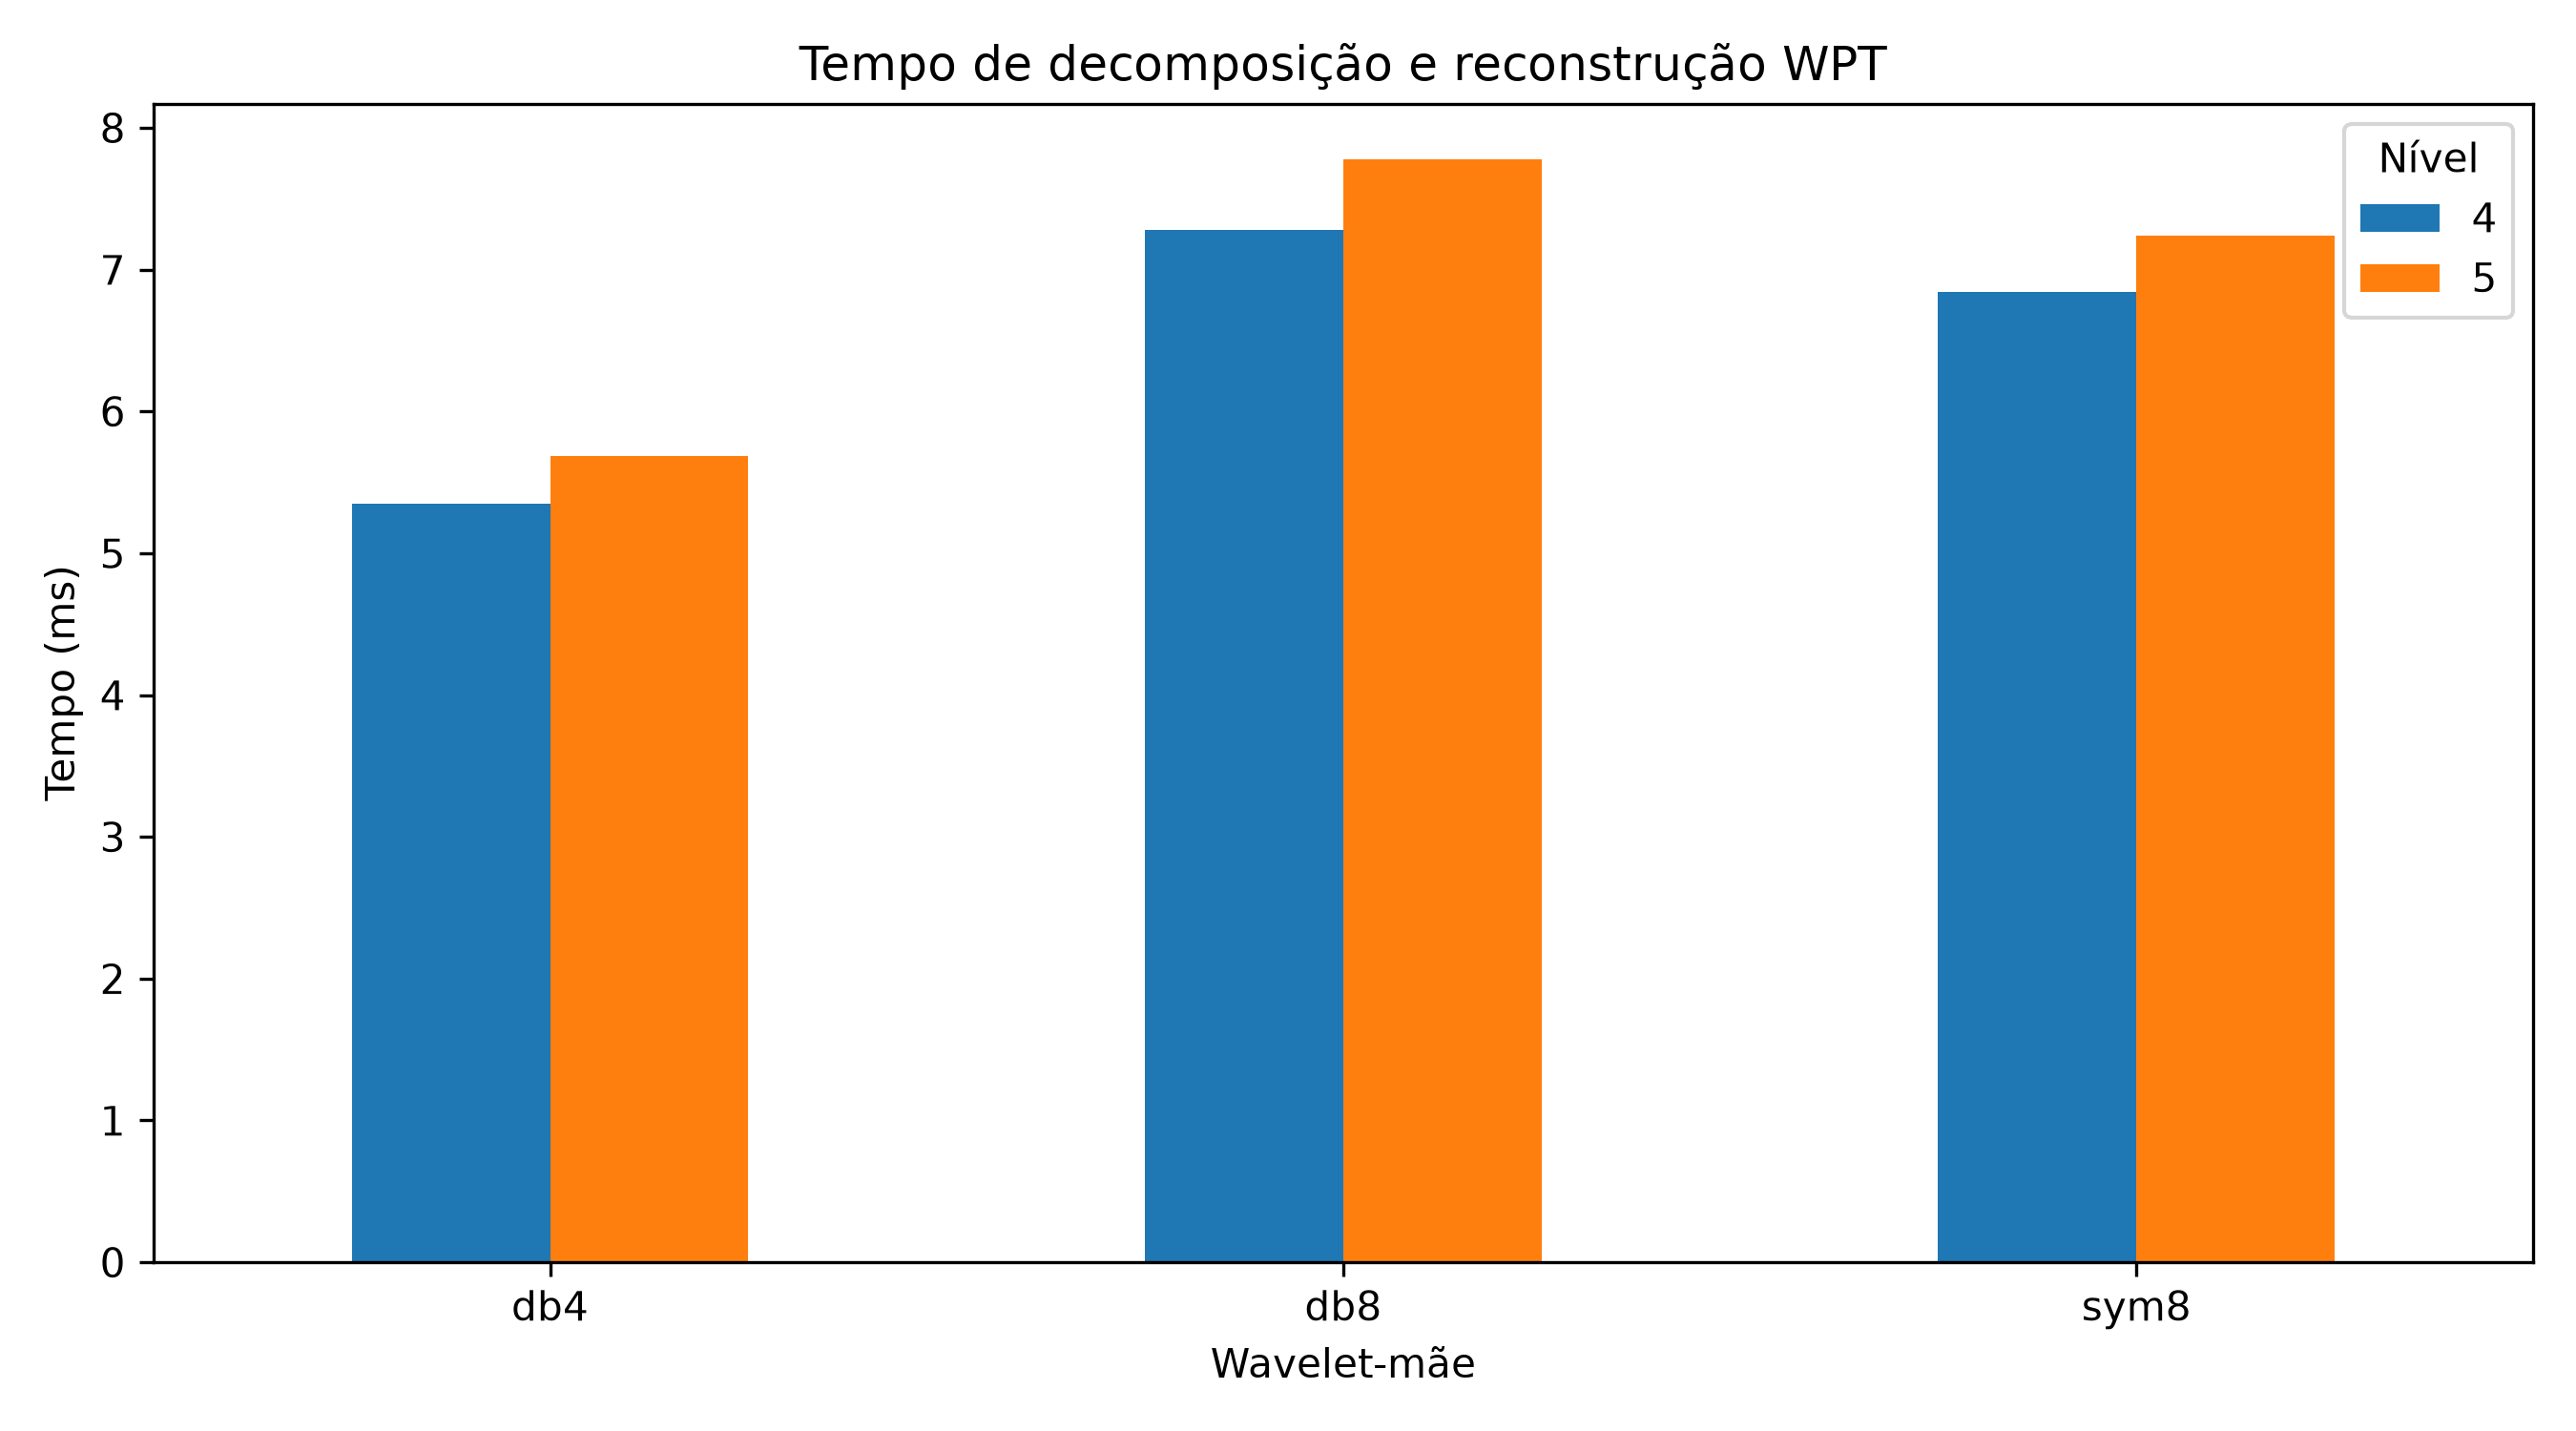
\includegraphics[width=0.95\textwidth]{figuras/comparacao_wavelets.png}
\caption{Comparação preliminar dos tempos de processamento WPT.}
\end{figure}

\begin{figure}[htbp]
\centering
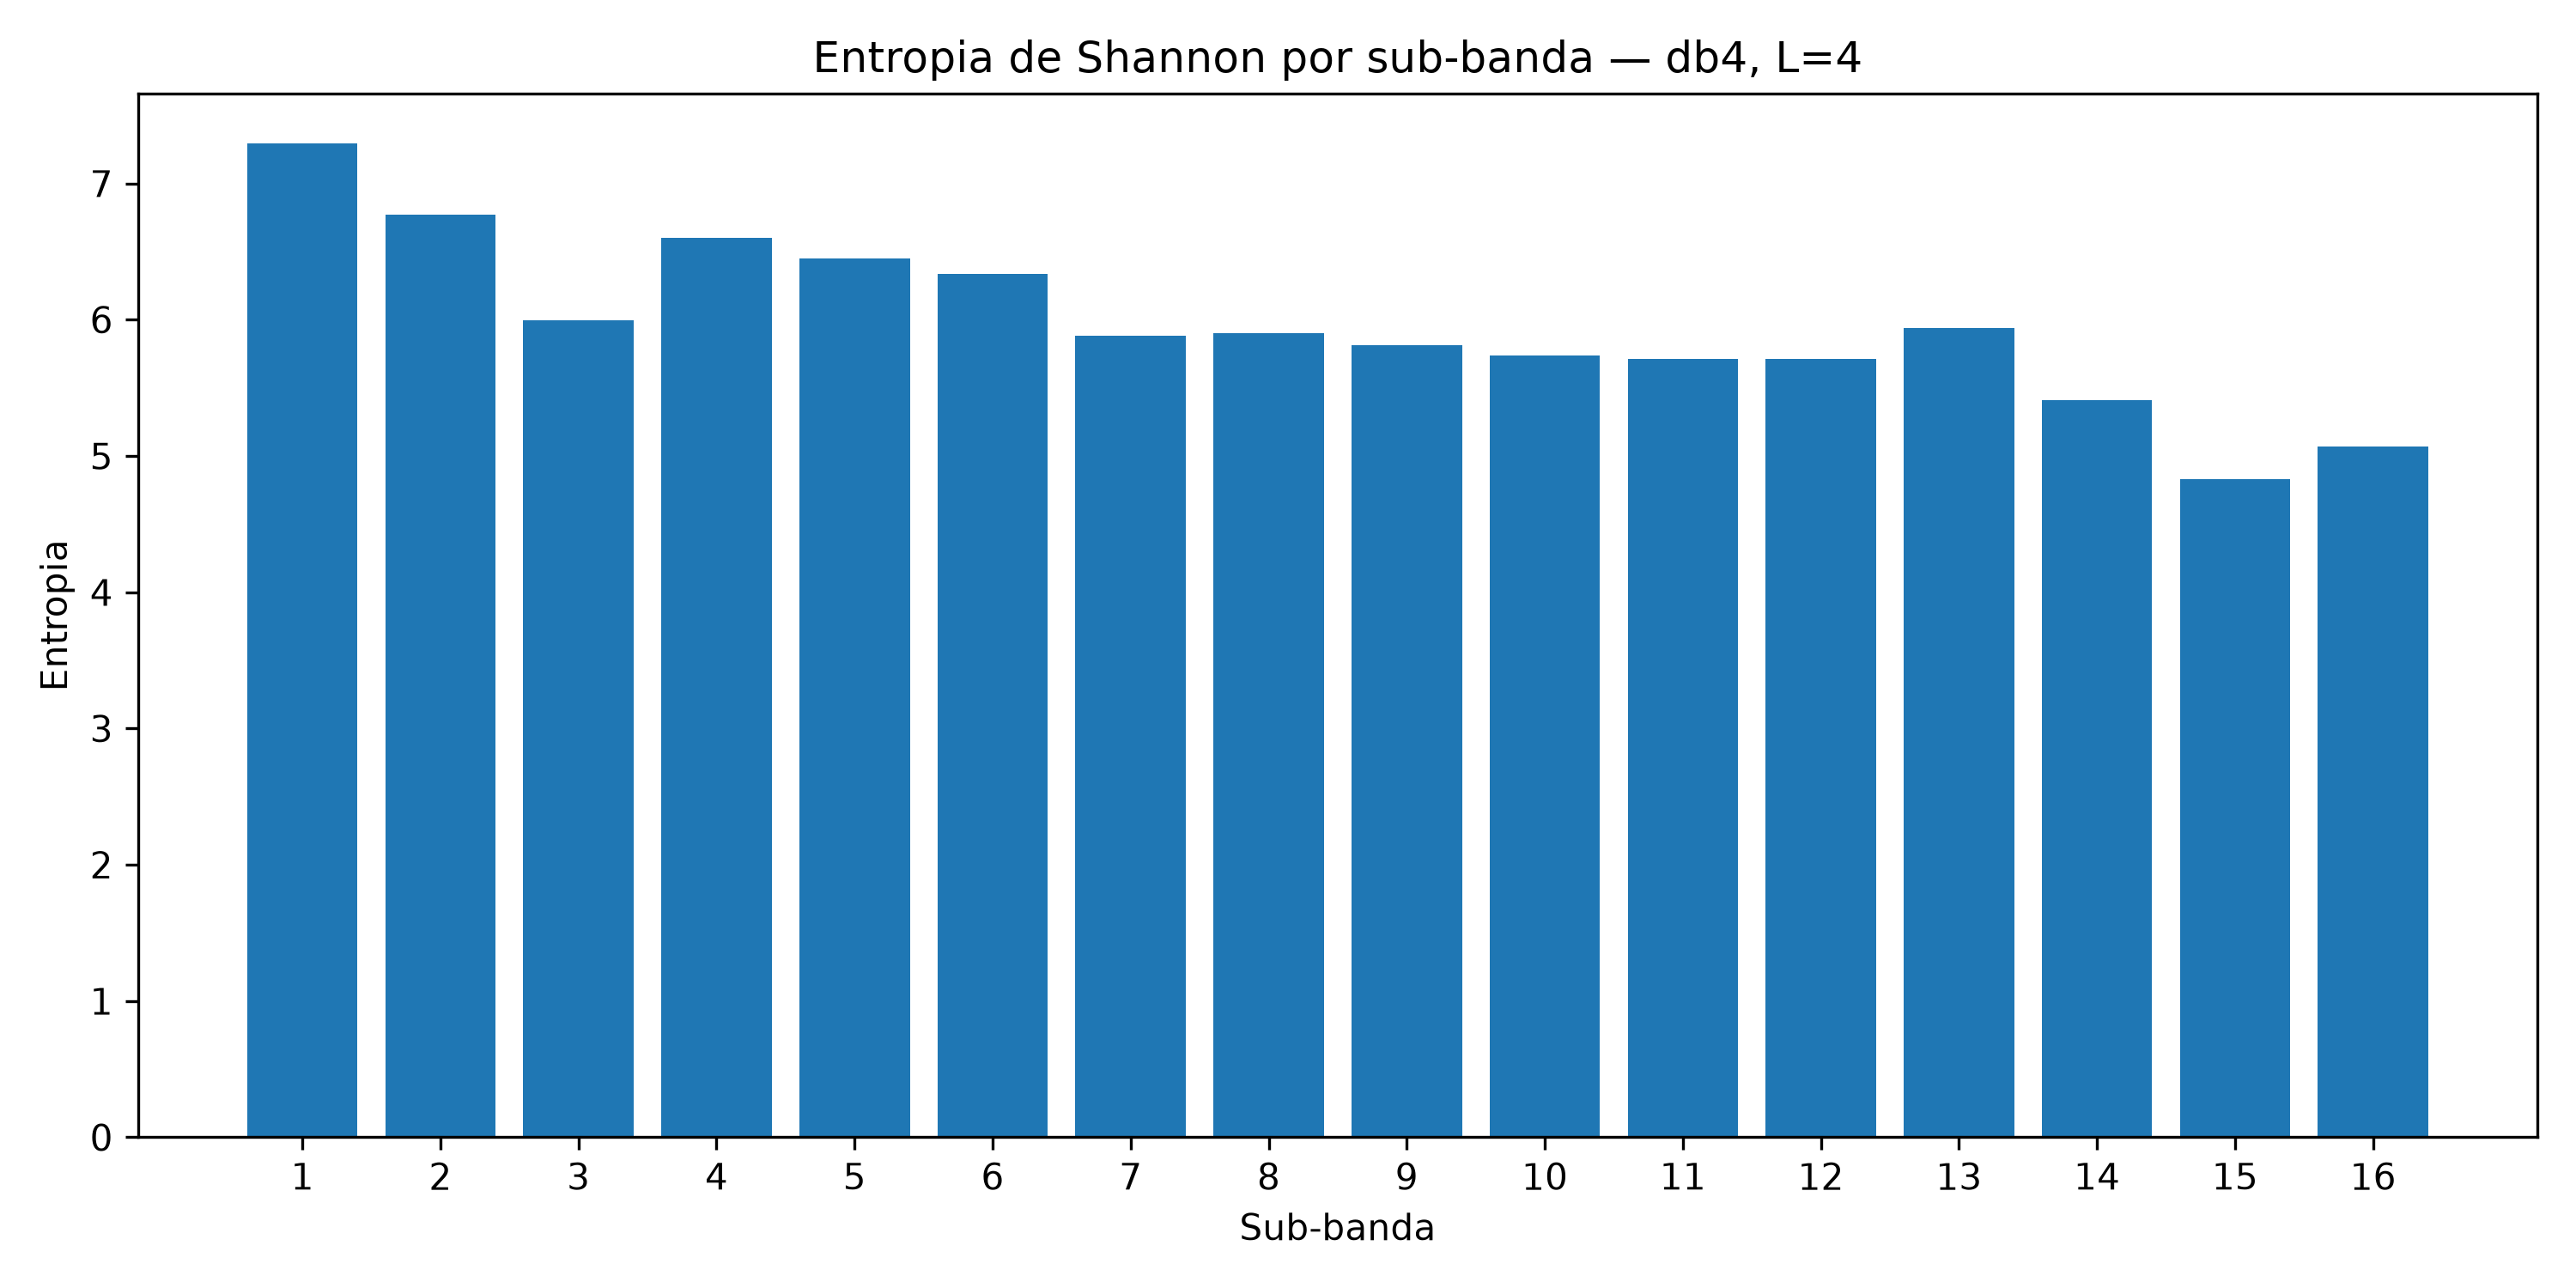
\includegraphics[width=0.95\textwidth]{figuras/entropia_subbandas.png}
\caption{Entropia de Shannon nas 16 sub-bandas do áudio real.}
\end{figure}

\begin{figure}[htbp]
\centering
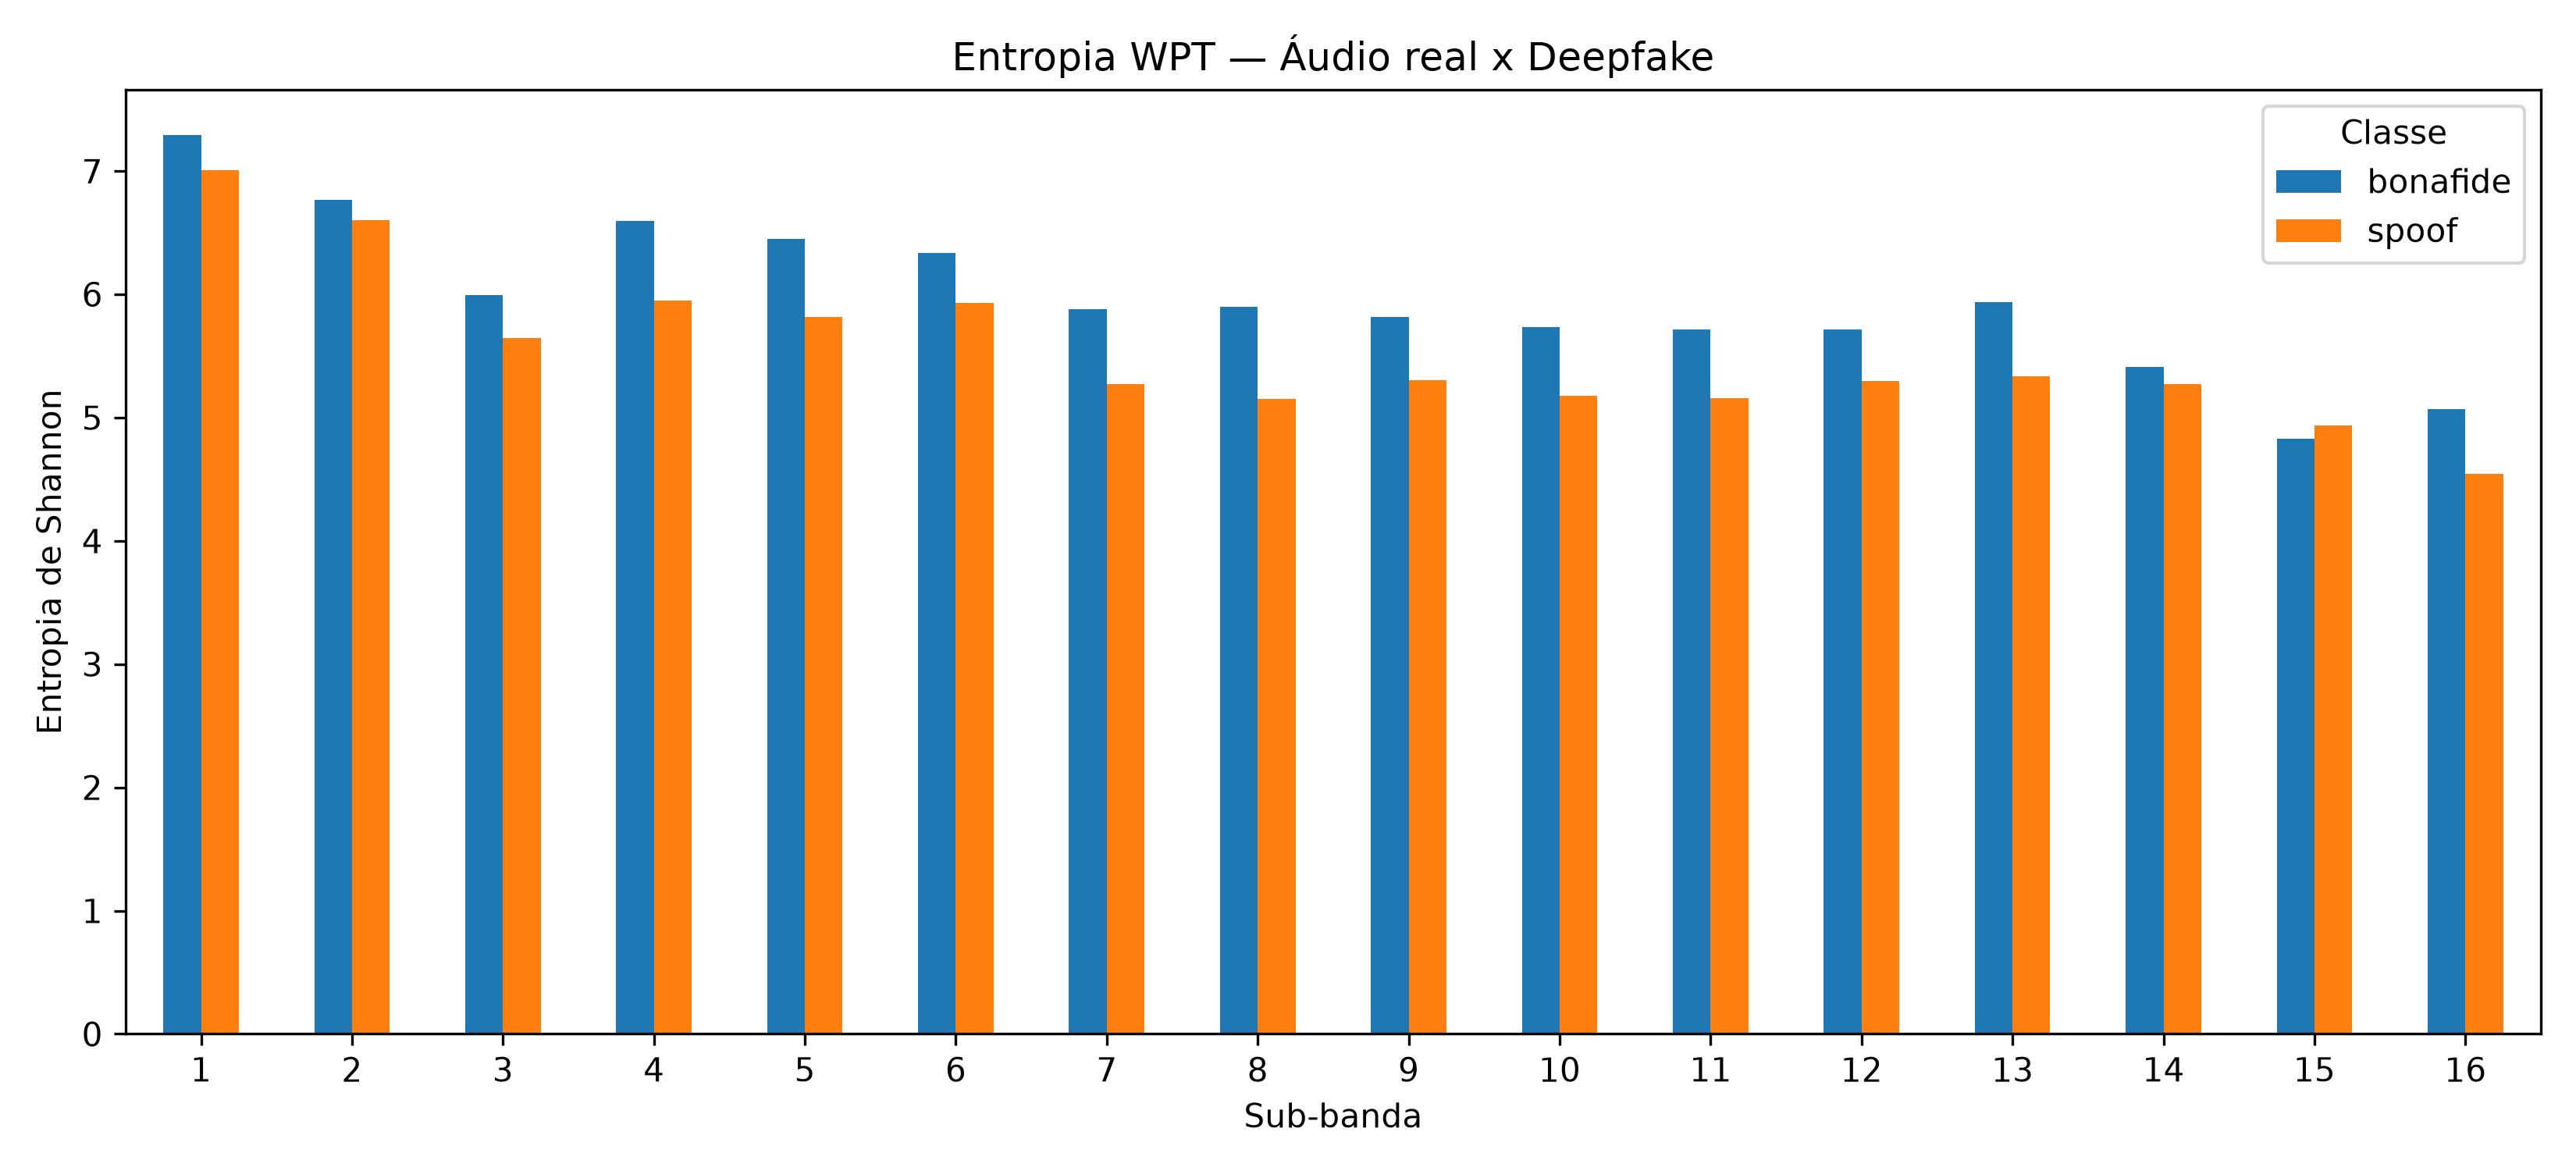
\includegraphics[width=0.95\textwidth]{figuras/comparacao_real_spoof.png}
\caption{Comparação exploratória de entropia entre áudio real e sintético.}
\end{figure}


\end{document}
